
\graphicspath{ {\curdir/Graphics/}  }

As we make progress towards effectively cooling these ion chains we want to begin exploring how quantum operations can be engineered in them.  We have begun performing single qubit quantum gates with barium ions in our system, and are preparing the necessary infrastructure to being characterizing entangling gates.  Currently, our single qubit gates are driven with resonant rf fields, but we are developing a Raman laser system to perform these gates that will have single qubit addressability and large enough Lamb-Dicke parameter to also perform two qubit entangling gates.  We will begin by characterizing these gates in barium ions in our mixed species chains, but eventually transition to the architecture described previously.

\section{Zeeman Transitions}
\label{sec:zeeman}

The Zeeman qubit I have described in barium, as well as the hyperfine qubit in ytterbium, can be coherently controlled by applying rf or microwave magnetic fields to the ions.  In our group we have some traps that have been designed to accommodate applying large amplitude oscillating magnetic fields to ions by placing copper transmission lines along paths inside of the vacuum chamber near the ion.  Our current quantum information vacuum chambers were not designed to incorporate this feature, and for the moment we are applying the fields from the outside.

We have demonstrated our ability to find and drive Zeeman transitions in single barium ions using an external field coil driven by a Stanford SRS-345 frequency source.  The field coil is composed of approximately 20 turns of copper wire and is located on our imaging viewport approximately 1~cm from the ion.  The rf can be crudely coupled onto this coil by making a resonant circuit by adding capacitance to cancel the inductance of the coil near the Zeeman transition frequency.

The experimental procedure to observe these transitions again begins by switching the cooling lasers to perform optical pumping and pumping the ion into the $m_J = -\frac{1}{2}$ level of the ground state. The cooling lasers are then shuttered and we attempt to drive a Zeeman transition by applying resonant rf at our Zeeman transition frequency $\omega$ = $2 \pi \times$ 14.610~MHz to the field coil.  After this attempt, we apply a $\pi$-pulse of 1762~nm light to drive the $m_J = -\frac{1}{2}$ level to the $m_J = -\frac{1}{2}$ level of the 5D$_{5/2}$ shelved state with a probability of approximately 90\%.  Finally, we reactivate the cooling lasers and the ion fluoresces if it has not been successfully shelved.

For our initial characterization of this process, we have only been able to apply relatively small magnetic field amplitudes to the ion.  Figure~\ref{fig:zeeman-rabi} shows the shelving probability as a function of the exposure time of our rf source.  The beginning of a Rabi oscillation is clear, but then the frequency and amplitude of the transition begin to change.  These changes are due to the changing magnetic field in the trap because of the changing ac wall phase.  All of our magnetically sensitive experiments are triggered to begin on a maximum of the ac wall voltage, but since this experiment lasts for several milliseconds we begin to see the magnetic field shift.  Without magnetic shielding it is almost impossible to avoid having a large changing magnetic field caused by the current draw of all of the lab electronics.

\begin{figure}
	\centering
	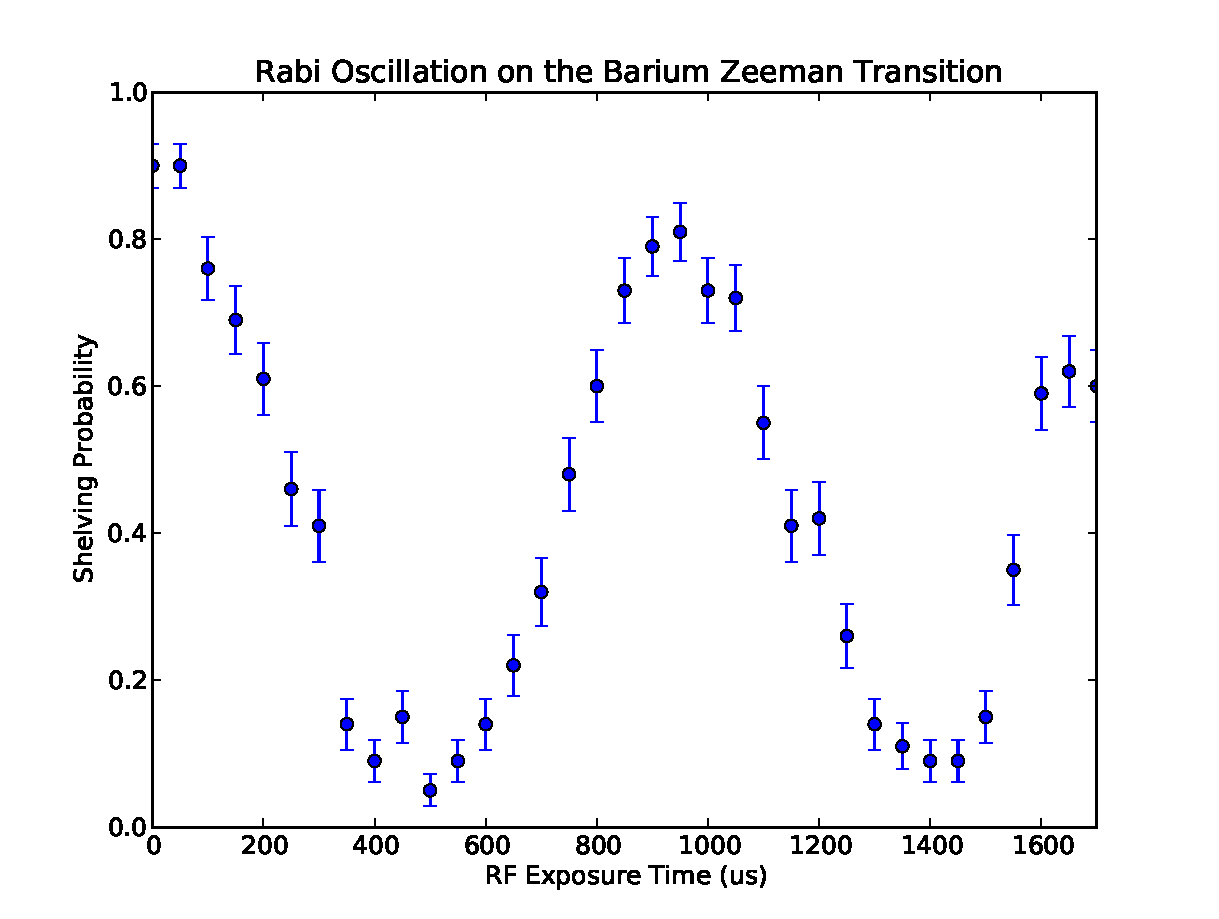
\includegraphics[width=0.8\textwidth]{ZeemanRabi}
	\caption[Rabi oscillations between Zeeman levels of the ground state of \ba]{Rabi oscillations between the \ba ground state Zeeman levels.  The probability of driving a 1762~nm transition from the Zeeman level the ion was initialized to is shown as a function of exposure time of rf current resonant with the Zeeman energy splitting.  The complicated behavior is caused by magnetic field shifts from the ac wall current.}
	\label{fig:zeeman-rabi}
\end{figure}

The fidelity of this qubit operation is currently low in our setup, but it demonstrates that we have the infrastructure to support these kinds of operations.  In other traps, my group has shown Rabi oscillations between these levels with 600~ns $\pi$-pulses and fidelities greater than 99\%. The fidelity in our setup could be quickly improved by using amplifiers and resonators to apply a stronger magnetic field to the ion.  Increasing our magnetic field would decrease the gate operation time and significantly reduce the size of the magnetic field drift.  Our maximum shelving probability could also be significantly improved by carefully improving our optical pumping efficiency and the 1762~nm $\pi$-pulse fidelity.  In actual quantum information processing, we plan to drive our single qubit gates using optical Raman transitions and therefore it is not necessary to optimize the fidelity of these rf-driven gates.  

\section{Raman Transitions}
\label{sec:raman-trans}

The difficulty with performing qubit rotations using resonant rf or microwaves is that the energy separation between ideal qubit levels can often be very small.  Therefore, near resonant radiation will have a long wavelength and be difficult to address onto single ions.  For example, the hyperfine qubit in $^{171}$Yb$^+$ has $\omega =$ 12.643~GHz, which corresponds to a wavelength of approximately 2.5~cm.  Typical ion separations in a single trapping region are 5~um to 10~um.  For performing quantum algorithms where we need to perform different rotations on adjacent qubits, we will need to use different techniques.  

It is possible to generate spatially varying microwave field intensities on the micron level using several electrodes on a surface trap geometry which enables single qubit addressing \cite{Warring:13}.  The energy difference of the qubit levels can also be varied by applying large magnetic field gradients to ion chains which enables frequency addressing single qubits \cite{Wang:09}.  Both of these techniques involve adding control electrodes to surface traps, but can achieve reasonably low crosstalk of a few percent or less.

We are planning to instead use optical Raman transitions to implement single- and multi-qubit gates.  Using optical Raman transitions is advantageous because the lasers driving them can easily be focused onto individual ions, and the photons absorbed and emitted carry enough momentum to usefully couple to the motion of the ions.  The interaction between optical fields and the motional modes of the trap is still characterized by the Lamb-Dicke parameter $\eta$ = $k_\mathrm{photon} x_\mathrm{ion}$.  We are planning to use a 532~nm laser to drive these transitions on our $\approx$ 1.2~MHz radial motional modes, which results in $\eta \approx$ 0.05.

\begin{figure}
	\centering
	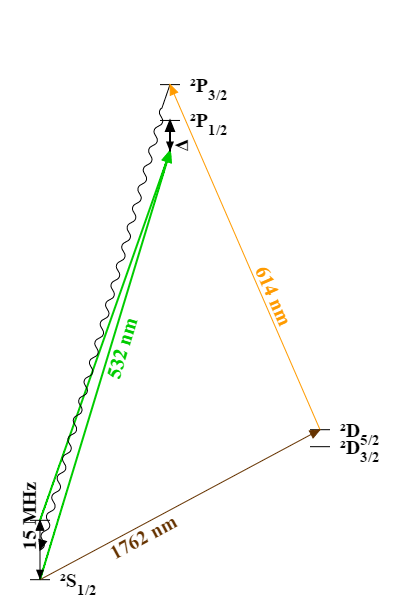
\includegraphics[width=0.5\textwidth]{ba-qcomp-lasers}
	\caption[Energy level diagram of Ba$^+$ quantum computation lasers]{Energy level diagram of Ba$^+$ including ground state Zeeman levels (not to scale) and relevant lasers.  Raman transitions can be driven using two 532~nm beams with a relative detuning equal to the Zeeman energy spacing.  Readout will still be performed using the 1762~nm laser.}
	\label{fig:ba-qcomp}
\end{figure}

For a pair of monochromatic light fields the Rabi frequency for Raman transitions can be written as 
\begin{equation}
	\Omega = \frac{ \left| \vec{\mu}_1 \cdot \vec{E}_1 \right| \left| \vec{\mu}_2 \cdot \vec{E}_2 \right| }{ \hbar^2 \Delta } \mathrm{,}
\end{equation}
where $\vec{\mu}_i$ are the electric dipole moment coupling the two Zeeman qubit levels to an intermediate level in the 6P$_{1/2}$ or 6P$_{3/2}$ state, $\vec{E}_i$ are the electric field magnitude and polarization for the two beams, and $\Delta$ is the detuning of each beam from the excited state.  Our detunings $\Delta$ are $2 \pi \times$ 44.5~THz from the 6P$_{1/2}$ state and $2 \pi \times$ 95.4~THz from the 6P$_{3/2}$ state.  However, our 532~nm source is not monochromatic, since the light is provided by a mode-locked laser.

The electric field from a mode-locked laser can be described by
\begin{equation}
	\vec{E}(t) = \vec{E}_0 \sum\limits_{n=0}^\infty f( t - n T ) \cos( \omega t + k_x x )
\end{equation}
where $\vec{E}_0$ is the electric field magnitude and polarization, $\omega$ is the center frequency of the laser, the function $f$ describes the pulse shape of the laser, and $T$ is the time period between pulses.  In an optimal mode-locked laser, $f(t) \propto \sech( \pi t / \tau )$, where $\tau$ is the time duration of the pulses.  Taking the Fourier transform of this field we can find that it has many sharp spectral components separated by the repetition rate of the laser, $\omega_R = 2 \pi / T$, in a $2 \pi / \tau$ bandwidth around $\omega$.  These ``comb teeth'' can be used to drive narrow atomic transitions \cite{Hayes:10}.  The frequency width of these teeth, $\omega_R / N$, is controlled by the number of pulses, $N$, applied to the ion.

\begin{figure}
	\centering
	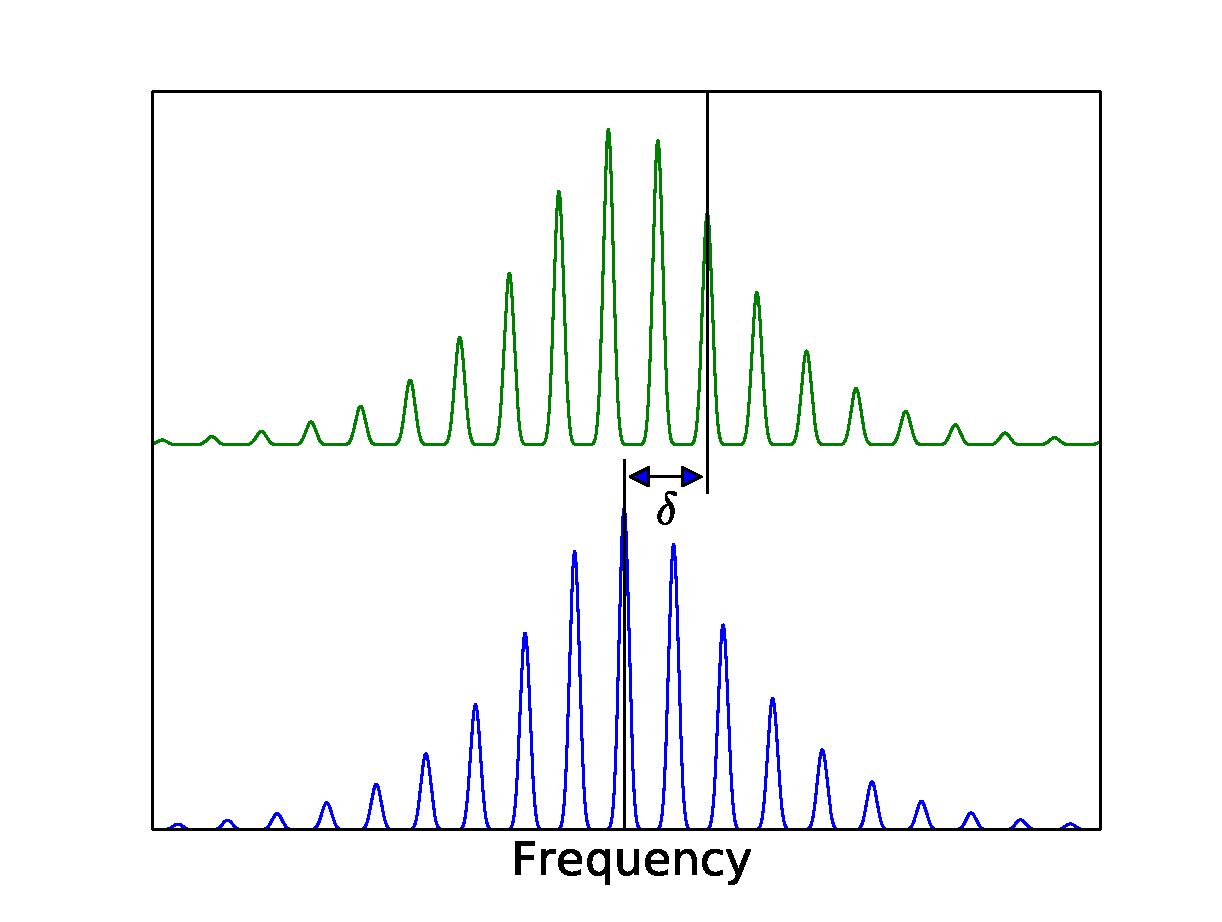
\includegraphics[width=0.7\textwidth]{ModelockedSpectrum}
	\caption[Frequency spectrum of a series of pulses from a modelocked laser]{Frequency spectrum of a series of pulses from a modelocked 532~nm laser.  The comb teeth are spaced by the repetition rate of the laser, and can be made more narrow by applying more sequential pulses to the ion.  The two pulse trains are detuned from one another by an AOM, and Raman transitions can be driven for any frequency $\delta$ equal to a multiple of the repetition rate plus or minus the AOM frequency.}
	\label{fig:modelocked}
\end{figure}

We will be using these comb teeth to drive Raman transitions between our qubit levels.  Therefore we require that the bandwidth of the laser is significantly larger than our qubit energy spacing such that many of the comb teeth can contribute to driving the transition.  By independently frequency shifting two beams from the laser by $\delta$, we will tune their frequency difference such that $\omega_\mathrm{qubit} = m \omega_R + \delta$ for some integer $m$. The resulting Raman transition will have a coupling strength given by
\begin{eqnarray}
	\Omega &=& \sum_n \frac{ \mu^2 E_n E_{n-m} }{ \hbar^2 \Delta } \\ 
	&\approx& \frac{\omega_R \tau}{2\pi} \frac{\mu^2 E_0 ^2}{\hbar^2 \Delta}
	\label{eqn:ramanapprox}
\end{eqnarray}
where $E_n$ is the electric field magnitude of comb tooth n and can be found from f.  The approximation is valid when $\omega_\mathrm{qubit} \tau \ll 1$ such that most of the comb teeth have a corresponding comb tooth at the correct detuning.  By simultaneously driving two Raman transitions with detunings of $\omega_\mathrm{qubit} \pm \delta$ on two ions, with $\delta \approx \omega_x$, we can use this laser to generate entanglement between ions using the M{\o}lmer-S{\o}rensen gate.  For our 532~nm light driving Raman transitions in barium, we must consider coupling through both the 6P$_{3/2}$ and the 6P$_{1/2}$ state.  We estimate that given our current laser power and focusing constraints, we can expect to drive carrier Raman transitions at a rate of $\Omega \approx$ 50~kHz.  The M{\o}lmer-S{\o}rensen coherent two qubit operation can be driven at a rate of $2 \eta \Omega \approx$ 5~kHz.

We will be using a mode-locked diode-pumped ND:YVO$_4$ laser to provide the optical beams.  This laser was originally a multimode CW pump laser for a Ti:Sapphire mode-locked laser, but it has been modified to support mode-locked operation itself.  Mode-locked operation is favored by a semiconductor saturable absorber end mirror that has been added to the laser cavity.  In addition, the cavity had been modified to produce the necessary tight focus on the saturable absorber \cite{Schlatter:04, Sun:10}.  The laser produces 2~W of optical power at 1064~nm that we frequency double using a LBO crystal in a single pass configuration to 500~mW of 532~nm light.  The output pulses were measured using an autocorrelator to have 17~ps duration and our repetition rate is approximately 150~MHz.

In order to drive Raman transitions using this system we need to split the pulse train into two beams and frequency detune these beams from each other (see Figure~\ref{fig:modelocked}).  We have accomplished this using two AOMs.  A base 220~MHz signal is generated by an HP-8640B signal generator and then split into two paths by a rf power splitter.  One path continues directly to a high speed rf switch, while the other is mixed with a computer controlled Stanford Research Systems DS345 20~MHz signal generator, resulting in signals at 200~MHz and 240~MHz, and then sent to a different switch.  Both paths are then amplified to approximately 1~W and sent to separate 200~MHz AOMs.  The bandwidth of the amplifier and the AOM severely attenuates the 240~MHz signal from the mixer leaving the two AOMs to be driven by 200~MHz and 220~MHz signals, respectively.  The common mode 220~MHz signal has no effect on Raman transitions and so the stability only depends on the DS345 signal and there is no need to phase lock two rf sources together.  This optical setup is operational with both beams controlled by the AOMs and focused into the trap.  The path length difference between the two beams is set by a linear delay stage and has been measured to approximately overlap the pulses in from the two paths.  Since we know the energy separation of the Zeeman levels because we have directly driven the the transition between them, there are no remaining degrees of freedom in the system.  We expect to observe optical Raman transitions very soon.

In the future we plan to provide the rf for the two Raman beams with a two channel DDS system based on the Analog Devices AD9958 part.  The two channels are controlled through a serial interface and are phase coherent because they are created from the same reference clock.  This device will also allow us to provide feedback to stabilize the frequencies of the comb teeth against path length drift in the optical cavity.  We will also be able to program pulse sequences with different amplitudes and phases into the DDS to perform error-compensating pulse sequences \cite{Hayes:12}.

These techniques have been developed using commercial systems by several other ion trapping groups.  M{\o}lmer-S{\o}rensen gates with 10 to 100~$\mu$s $\pi$ time have been developed \cite{Hayes:10}.  The bandwidth of the modelocked laser we have built ($\approx$ 100~GHz) is also sufficient to span the 12.6~GHz hyperfine splitting in ytterbium ions to drive entangling gates between these levels.  As we develop our ability to work with quantum information in ytterbium, this laser will become increasingly important.  We can use a second nonlinear crystal to generate light at the third harmonic of the laser frequency at 355~nm, which is at an optimal frequency detuning for driving Raman transitions in ytterbium \cite{Campbell:10}.

\section{Conclusions and Outlook}
\label{sec:conclusions}

The initial infrastructure for working with mixed species ion chains in a quantum computer architecture has been described here and implemented in my lab.  We have developed the technology that we will use to work with surface electrode ion traps in the future.  We can simulate the effect of applying dc voltages to these traps using simulation tools and apply sequences of voltages quickly with a FPGA driven DAC system.  These traps will be able to stably confine more ions in each trapping region and hold multiple separate trapping regions within the same vacuum chamber.  The additional voltage degrees of freedom will give us greater control over the trapping potential the ions experience within each trap.  We have demonstrated using these systems to shuttle ions around the surface trap and perform experiments in different locations to explore the local features of these traps.  Initial measurements of secular frequencies, stray fields, and heating rates have been made that will guide us in improving our cooling and trapping apparatus in the future.

We can repeatably ionize, trap, and cool barium and ytterbium ions.  Currently the temperature of the normal modes that are strongly coupled to the ytterbium ions will be problematic for implementing entangling gates, but there are many possible avenues for overcoming this problem.  The temperature measurement techniques we have developed will allow us to optimize our cooling and trapping parameters.  One of the main difficulties in performing these experiments at the moment is that in our macroscopic Paul trap the ordering of the ions is random.  As we move the techniques we have developed to surface electrode traps, we should be able to perform experiments with tens of ions and full control over the number and configuration of the cooling ions.  We will then be able to fully investigate the scalability of this architecture.

Lastly, although most of my work has gone into the basic trapping and cooling infrastructure for our scalable system,  we have made some progress towards performing actual quantum gates using this system.  We have found and driven our Zeeman qubit level in \ba, which will enable us to rapidly set up our actual quantum operations experiments with our mode-locked laser.  We have fully characterized the performance of this laser and we are beginning experiments to attempt to drive carrier transitions with it.  This system will allow us to begin testing how well all of the infrastructure we have developed will work during actual quantum computation.  That is an exciting step.

Overall the future for trapped ion quantum computing still looks promising.  All of the required basic systems have been implemented, and the only remaining challenge is having a sufficient number of communicating ions.  As you most certainly know by now, there are a huge number of different ways we can approach this goal.  We have been simultaneously working in several directions on this problem, and as we begin to combine these ideas into larger systems I think we'll be able to achieve some really amazing things.

